\documentclass[conference]{IEEEtran}
\IEEEoverridecommandlockouts
% The preceding line is only needed to identify funding in the first footnote. If that is unneeded, please comment it out.
\usepackage{cite}
\usepackage{amsmath,amssymb,amsfonts}
\usepackage{algorithmic}
\usepackage{graphicx}
\usepackage{textcomp}
\usepackage{xcolor}
\def\BibTeX{{\rm B\kern-.05em{\sc i\kern-.025em b}\kern-.08em
		T\kern-.1667em\lower.7ex\hbox{E}\kern-.125emX}}
\begin{document}
	
	\title{A Brief Survey on Text to Image Generation using Generative Adversarial Networks\\
	}
	
	\author{\IEEEauthorblockN{Ayushi Ahjolia}
		\IEEEauthorblockA{\textit{Electrical and Computer Engineering} \\
			\textit{University of Waterloo}\\
			Waterloo, Ontario \\
			ahahjoli@uwaterloo.ca}
		\and
		\IEEEauthorblockN{Deep Jariwala}
		\IEEEauthorblockA{\textit{Electrical and Computer Engineering} \\
			\textit{University of Waterloo}\\
			Waterloo, Ontario \\
			djariwal@uwaterloo.ca}
		\and
		\IEEEauthorblockN{Kavya Garikapati}
		\IEEEauthorblockA{\textit{Electrical and Computer Engineering} \\
			\textit{University of Waterloo}\\
			Waterloo, Ontario \\
			kavya.garikapati@uwaterloo.ca}
	}
	
	\maketitle
	
	\begin{abstract}
	The evolution of deep learning and computer vision has solved many real-world problems like speech to text, image synthesis, biomedical signal analysis, and many more. Image synthesis is one of the most challenging problems which could be solved using a unique architecture known as Generative Adversarial Networks (GANs). Ian Goodfellow founded GANs to solve multimodality in his paper "Generative Adversarial Nets," \cite{b1} where the possibility of generating images using noise and image as input was accomplished. The idea of using GANs in computer vision was extended to many more applications, one of them being text to image synthesis. Since textual input contains many sentences and words that describe the image, it is a multimodal problem. The major problem tackled in the recent development of text-to-image synthesis is generating high-quality images and converging the objective function at the global minimum. In this paper, we have reviewed the evolution of GANs architecture over the years to improve text to image synthesis. In this paper, we compared new ideas and architectures different from state-of-the-art models and compared their results.
	\end{abstract}
	
	\begin{IEEEkeywords}
		Generative Adversarial Networks, Text-to-Image synthesis, Generator, Discriminator, Min-Max Optimization, Computer Vision, Natural Language Processing.
	\end{IEEEkeywords}
	
	\section{INTRODUCTION}
	
	The advances in Machine learning and Artificial Intelligence gave rise to many new fields of study. Natural Language Processing (NLP) and computer vision are areas that found themselves helpful in a wide range of applications. NLP can be used in many applications; generating image descriptions is one of the most challenging problems. The inverse of this problem is developing an image by text description. All the deep learning models encountering this problem face conditional multi-modality, The mentioned task can be achieved using  Generative Adversarial Networks (GANs) which is a natural application for conditional multi-modality. It uses two entities, namely 1) Generator and 2) Discriminator. The generator generates images and attempts to fool the discriminator into believing that the created images are real. Given a picture, the discriminator attempts to detect whether it is real or synthetic. The assumption is that both players will improve by playing this game repeatedly, implying that the generator will learn to make realistic visuals. A way to visualize this is to define a game where we have an objective function O, a function of D and G, discriminator, and generator, respectively.  In the case of GANs, min-max optimization is used where the discriminator seeks to maximize O, whereas the generator seeks to minimize it. So, if the O is high, then the discriminator is guessing correctly, and if it is low, the generator is fooling the discriminator by synthesizing images that are not distinguishable from the real images. GANs solve most of the shortcomings of the already existing generative models:
	\begin{itemize}
		\item The quality of the image generated is better.
		\item It can generate samples efficiently and in parallel
		\item It is flexible in terms of choosing a loss function and topology of the network.
	\end{itemize}
	In general, GANs is the ideal approach for image synthesis, but has some shortcomings like:
	\begin{itemize}
		\item GAN training is relatively stable on some specific architectures with carefully chosen hyper-parameters.
		\item Often, GAN reaches a point of instability during training and lacks any indication for convergence.
		\item The best working GAN is far from the ideal assumed model.
	\end{itemize}
	
	The text descriptions must be vectorized to text embeddings, particularly for text to image synthesis instead of noise. Now, in the case of image synthesis derived by textual input, a pair of text embedding and the image is sent as an input to the discriminator. Now, in this case, the discriminator will have one more additional responsibility to predict the likelihood of whether the given text and image are aligned with each other, along with identifying whether the image is fake or real. The most recent methods for Text-to-Image (T2I) makes progress in increasing the resolution and visual quality by assembling a series of generator discriminator pairs to generate an image from coarse to fine details. This leads to a higher computational power, but it has been resolved by one stage generator proposed in the literature \cite{b1}. T2I models have other limitations of fusing the text embeddings and image information effectively. Generally, there are three main approaches to cross-modal attention, Condition Batch Normalization (CBN) and feature concatenation. This survey paper shows how the T2I model has been improved over the years for text-to-image synthesis. Moreover, We have demonstrated a comparative study between different architectures of GANs to illustrate the image synthesis.
	
	
	\section{LITERATURE REVIEW}
	
	Image synthesis from textual description using GANs have gained popularity in natural language processing and computer vision due to its unique properties and mathematical interpretations. The section will understand other literature emphasizing text to image using GANs.
	
	Reed et al.\cite{b2} published the state-of-art paper for text to image synthesis. In the above literature, the authors divided the problem in two major sub problems: finding a visually discriminative representation for text embeddings and use these embeddings to generate images which are close to reality. For the first sub problem, they used char-CNN-RNN encoder followed by conditional GANs to solve the next sub problem, which was named as Generative Adversarial Network- Conditional Latent Space (GAN-CLS). The GAN-CLS has a different cost/loss function where the goal is to better impose the text-image mapping on discriminator by making it aware about the text-image relationship. Impressively, the author merged the idea of generating large amount of additional embeddings using manifold interpolation (INT) method to improve the results. The final model which provided impressive results was GAN-INT-CLS. The disadvantage of GAN-CLS, failed to produce high resolution images is solved by StackGAN \cite{b3}.
	
	The StackGAN architecture uses two stages of GAN, stage 1: generates images from textual description at a lower resolution where as stage 2: has a generator which accepts the images generated by stage 1 as input data to produce a higher resolution resized image with more fine-grained details and better text-image matching. The authors in literature [reference] have showed the improved version of StackGAN known as StackGAN-v2 which uses multiple generators and discriminators in a tree like structure. Another significant contribution made in this field is made by authors in paper \cite{b3} where they proposed AttnGAN. AttnGAN and StackGAN-v2 have similar architecture, but with an attention model over it. The attention model has an advantage which creates a similar behavior to human mechanism and allows the network to process a single word from a sentence or a specific region of an image.
	
	Zhang et al. in his paper \cite{b4} has improved training  of text to image model using mode seeking function. In this paper,the problems with mode collapsing have been discussed and solved impressively by defining a dynamic memory GAN (DM-GAN). It learns the relation between text embeddings and images using a memory architecture to solve the multi modal problem. 
	
	The authors in the literature \cite{b5} have worked on two significant limitations of state-of-art T2I GANs (i) The CBN methods are applied on the whole image data's feature map equally, ignoring the local semantics (ii) The text encoder is fixed during the training with the image generator jointly to learn better text embeddings for image generation. The authors propose a novel Semantic-Spatial Aware GAN in the literature above, trained end-to-end to exploit better text information from the encoder. 
	
	
	
	\section{MATHEMATICAL INTERPRETATION}
	
	This section shows the mathematical framework for GANs. Let $\mathbb{X}$ be a dataset of samples $x^{i}$ belonging to a set of images in space $[-1,1]^n$. The discriminator learns a function $D_u$: $\chi$ $\rightarrow$ [0,1], which takes an image x and gives the probability it assigns to the images of being real. Let Z be the range of a random vector with a simple and definite distribution such as $p_\textbf{Z}$ = $\mathcal{N}$(0,I). The generator learns a function defined as $G_\theta$ : Z $\rightarrow$ $\chi$, which maps the states of the random vector X to Z. Thus, the generator learns to map a vector of noise to images. The easiest way to define and analyze GANs is through a game where $D_u$ and $G_\theta$ are the strategies of the two players. Such a game can be described by a objective/cost function O (D, G), which in this case represents the payoff of the discriminator. The discriminator wants to maximize the objective function while the generator wishes to minimize the same. The payoff described by the objective function O must be proportional to the ability of Discriminator to distinguish between fake and real samples. The image generated by the generator is based on a textual input distribution while the discriminator compares the generated image to the actual images. Thus adversarially, the discriminator uses the gradient obtained to train generator and the generator tries to fool the discriminator with the synthesis of image which is as close as possible to reality. Conditional GAN generates its output distribution with the the help of a directed input distribution based on an initial condition or context. The Fig. \ref{gan} shows the block diagram description of GANs. The objective function for min-max optimization for GANs is given by the equation below:
	
	\begin{equation}
	\begin{split}
	O(D,G) \hspace{0.2cm} = \hspace{0.2cm} \mathbb{E}_{\textbf{X}\sim\mathbb{P}_{r}}\hspace{0.1cm}[\log(D(x)]\hspace{0.2cm}+\\ \hspace{0.2cm} \mathbb{E}_{\textbf{\textbf{Z}}\sim p_{\textbf{Z}}}\hspace{0.1cm}[\log(1-D(G(z)))]      
	\end{split}
	\end{equation}
	
	\begin{figure}[htbp]
		\centering
		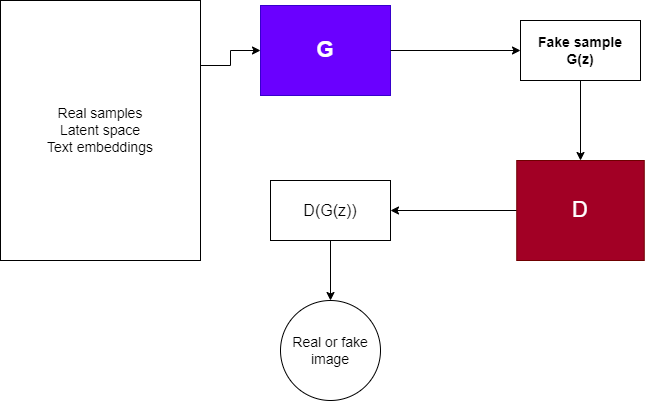
\includegraphics[width=0.35\textwidth]{GANS_final.png}
		\caption{Generative Adversarial Networks}
		\label{gan}
	\end{figure}
	
	The O(D,G) becomes higher when the discriminator can distinguish between real and fake samples. The reverse happens in when generator is performing well, the O becomes lower and cannot distinguish between real and fake samples. Here, $\mathbb{P}_r$ is the data generating distribution which produces the training dataset by sampling. The difference from maximum likelihood models is that samples generated by the generator having a distribution $\mathbb{P}_g$. The discriminator forces the generator to bring $\mathbb{P}_g$ close to $\mathbb{P}_r$. The optimization for GANs can be written by the equation below:
	
	\begin{equation}
	\theta \hspace{0.2cm} = \hspace{0.2cm} \frac{min}{G} \frac{max}{D} O(D, G)  
	\end{equation}
	
	Goodfellow [reference] proved that this minmax game reaches its global optimum when the distribution of generation is equal to distribution of dataset sampled. The solution to the above minmax optimization is provided by Nash Equilibrium. The nash equilibrim for GANs is obtained when,
	
	\[The \hspace{0.1cm} strategy \hspace{0.1cm} of \hspace{0.1cm} Discriminator \hspace{0.1cm} = \hspace{0.1cm} \frac{\mathbb{P}_r}{\mathbb{P}_r + \mathbb{P}_g} \]
	
	\[The \hspace{0.1cm} strategy \hspace{0.1cm} of \hspace{0.1cm} the \hspace{0.1cm} generator \hspace{0.1cm} makes \hspace{0.1cm} \mathbb{P}_r \hspace{0.1cm} = \hspace{0.1cm} \mathbb{P}_g\]
	
	
	
	\section{COMPARING ARCHITECTURES AND RESULTS OF DIFFERENT GANs}
	
	This section shows the architecture and results obtained by different GANs network. Moreover, we have formulated a comparative study to show the evolution in the concept of T2I using GAN.
	
	\subsection{GAN-INT-CLS}
	The network defined in this paper is the combination of a single generator discriminator pair. Initially, noise is sampled from Gaussian distribution and text query is encoded using text encoder \cite{b7}. Before this step the dataset is passed through manifold interpolation (INT) to increase the training samples. The embeddings is compressed to a smaller dimension using a fully connected layer followed by leaky-ReLU as activation. The result is merged with noise vector and fed to the generator. In the discriminator section, a block of stride, convolution with spatial batch normalization is formed which is connected to a leaky ReLU activation. The output of the generator is of the same dimension which is directly used as an input to discriminator. The performance of GANs, GAN-CLS, GAN-INT, GAN-INT-CLS is shown in the Fig. \ref{gan_int_cls}
	
	\begin{figure}[htbp]
		\centering
		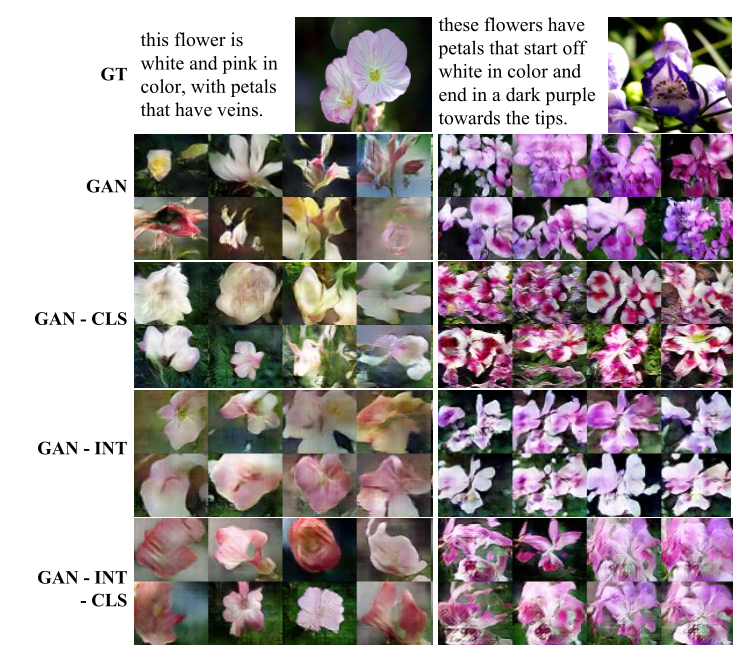
\includegraphics[width=0.45\textwidth]{GAN_cls_int.png}
		\caption{GAN-INT-CLS generated images \cite{b2}}
		\label{gan_int_cls}
	\end{figure}
	
	\subsection{Semantic-Spatial Aware GAN}
	The core elements for this architecture is Semantic-Spatial Aware Convolution network (SSACN) consisting of Semantic-Spatial Condition Batch Normalization (SSCBN) and a mask predictor. This transformation fuses the text embeddings with image features effectively, while encouraging the image features semantically consistent with	the text. The architecture consists of 3 stages: (i) Text encoder: it is bi-directional pre-trained model using text image pairs by minimizing Deep Attentional Multi modal Similarity Model (DAMSM) loss. (ii) Generator: it consists of stack of fully connected layer and SSACN. The SSACN is a complex block which contains a mask predictor that generates a mask of the image based on text to form a definite edge of the image and then based on the text embeddings the image is upsampled and fed to the discriminator. (iii) Discriminator: It is a one way structure that merges the encoded text with formed images from the generator though two convolution layers. In terms of results, it has acheived remarkable improvements over the T2I models with higher IS on all the images generated. Compared to DF-GAN and DM-GAN, this model fuses the text and images in a better way to capture the details of the text into the image formed. Fig. \ref{gan_SSAGN} shows the results and comparison obtained by this method. 
	
	\begin{figure}[htbp]
		\centering
		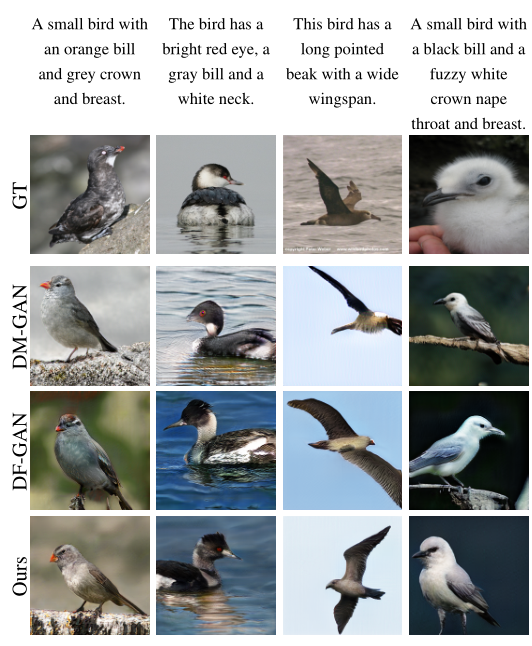
\includegraphics[width=0.40\textwidth]{GAN_SSAGAN.png}
		\caption{Results of SSA-GAN \cite{b3}}
		\label{gan_SSAGN}
	\end{figure}
	
	\subsection{Stack-GAN, Stack-GAN-v2}
	The purpose stacked GAN is to generate high-resolution images with finer details. Therefore, Stacked GAN consists of two stages: (i) Stage-I GAN: yields a low resolution image from the noise vector by drawing primitive shape, background color of the object based on text. (ii) Stage-II GAN: It performs completion of image by adding finer details to produce low to high resolution output. In the stage I, the text embeddings are fed into a fully connected layer to generate a Gaussian distribution with a fixed mean and standard deviation. Then, the dimension of the image is reduced and concatenated with text tensor and fed to 1x1 convolution. The discriminator consists of 1x1 convolution along with fully connected dense layer which produces a decision score. The stage II low resolution images are used as an input for converting them to high resolution. In the stage 2, the training method is different it maximizes the discriminator loss and minimizes the generator loss. Instead of using the random noise , Gaussian conditioning variables c used in this stage. It shows a clear improvement over state-of-the-art by 29 \%\ in terms of accuracy. Moreover, a significant difference is observed between stage I and stage II images as shown in Fig. \ref{gan_stack}.
	
	\begin{figure}[htbp]
		\centering
		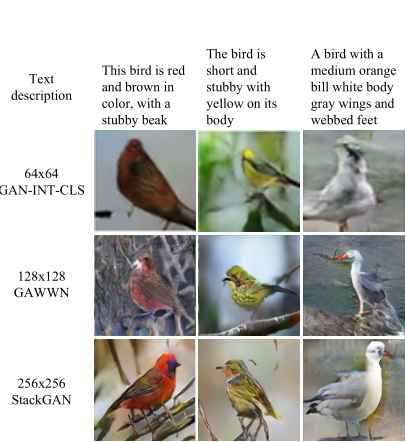
\includegraphics[width=0.45\textwidth]{stackGAN.png}
		\caption{Results of StackGAN \cite{b5}}
		\label{gan_stack}
	\end{figure}
	
	\subsection{DM-GAN}
	DM-GAN uses memory architecture to learn the fusion between image and text embeddings. The objective of dynamic memory is to fuse the image and text information between the value memory and key. The memory architecture is assembled in three forms: (i) Memory writing module, encodes prior information to image vectors and text vector by the means of convolution operator. (ii) Key addressing is used to search related memory using the similarity function. (iii) Value reading perpares the memory for output representation (iv) Response gate, it merges text with image.
	The mode seeking function defined here, calculates the ratio of the distance between the image vectors to the distance between normal vectors. The purpose for this addition is to separate the image vector and avoid overlapping to generate higher quality images. The regularization term forces the generators to explore more minor modes and varying its amplitude will result in a better image quality. The results obtained by this architecture is better in quality  with finer features and better characteristics. The parameter $\lambda$ is varied to change the mode seeking function and make better quality images. Fig. \ref{gan_dm} shows the effect of $\lambda$ over the quality of the image generated using DM-GAN.
	
	\begin{figure}[htbp]
		\centering
		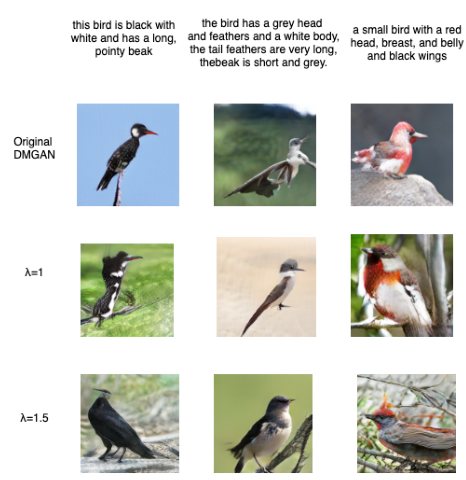
\includegraphics[width=0.45\textwidth]{DMGAN.png}
		\caption{Results of DMGAN \cite{b4}}
		\label{gan_dm}
	\end{figure}
	
	\section{CONCLUSION AND FUTURE PROSPECTS}
	It can be seen from the review that adding up more generator-discriminator pairs, changing the architecture, and improving the stability of GANs network have improved the quality and details of the images generated. Many architectures have evolved by incorporating more regularization techniques like adding a new mode seeking loss function, enhancing the input text embeddings, adding batch normalization, and adding mask generator have improved image quality without costing a significant computational power. The problem with GANs is the varnishing gradient due to the instability of the generator and discriminator network. Moreover, the mode collapsing problem is frequent, which is the current development in the text-to-image synthesis using GANs.
	
	\begin{thebibliography}{00}
		\bibitem{b1} an Goodfellow, Jean Pouget-Abadie, Mehdi Mirza, Bing Xu, David Warde-Farley, Sherjil Ozair, Aaron Courville, and Yoshua Bengio. Generative adversarial nets. In Z. Ghahramani, M. Welling, C. Cortes, N. D. Lawrence, and K. Q. Weinberger, editors, Advances in Neural Information Processing Systems 27, pages 2672–2680. Curran Associates, Inc., 2014..
		\bibitem{b2} Reed, Scott and Akata, Zeynep and Yan, Xinchen and Logeswaran, Lajanugen and Schiele, Bernt and Lee, Honglak, Generative Adversarial Text to Image Synthesis, Proceedings of The 33rd International Conference on Machine Learning, 2016.
		\bibitem{b3} Kai Hu and Wentong Liao and Michael Ying Yang and Bodo Rosenhahn, Text to Image Generation with Semantic-Spatial Aware {GAN}, CoRR, 2021.
		\bibitem{b4} Naitik Bhise and Zhenfei Zhang and Tien D. Bui, Improving Text to Image Generation using Mode-seeking Function, CoRR, 2020.
		\bibitem{b5} Zhang, Han and Xu, Tao and Li, Hongsheng and Zhang, Shaoting and Wang, Xiaogang and Huang, Xiaolei and Metaxas, Dimitris N., ``StackGAN: Text to Photo-Realistic Image Synthesis With Stacked Generative Adversarial Networks,'' Proceedings of the IEEE International Conference on Computer Vision (ICCV), Oct, 2017.
		\bibitem{b6} C. Wah, S. Branson, P. Welinder, P. Perona, and S. Belongie. The Caltech-UCSD Birds-200-2011 Dataset. Technical Report CNS-TR-2011-001, California Institute of Technology, 2011.
		\bibitem{b7}Scott Reed, Zeynep Akata, Bernt Schiele, and Honglak Lee. Learning deep representations of fine-grained visual descriptions. In IEEE Computer Vision and Pattern Recognition, 2016.
	\end{thebibliography}
\end{document}

